\documentclass[a0]{a0poster}
%A0 841mm x 1189mm
\usepackage{multicol} % This is so we can have multiple columns of text side-by-side

\usepackage[svgnames]{xcolor} % Specify colors by their 'svgnames', for a full list of all colors available see here: http://www.latextemplates.com/svgnames-colors

%\usepackage{times} % Use the times font
%\usepackage{palatino} % Uncomment to use the Palatino font
%\usepackage[sfdefault]{AlegreyaSans}
\usepackage[sfdefault]{AlegreyaSans}

\usepackage{graphicx} % Required for including images
\graphicspath{{figures/}} % Location of the graphics files
\usepackage{booktabs} % Top and bottom rules for table
\usepackage[labelfont=bf]{caption} % Required for specifying captions to tables and figures
\usepackage{amsfonts, amsmath, amsthm, amssymb} % For math fonts, symbols and environments
\usepackage{wrapfig} % Allows wrapping text around tables and figures
\usepackage{bm}
\usepackage{ragged2e}
\usepackage{float} % para que los gr\'aficos se queden en su lugar con [H]
\usepackage[subrefformat=parens]{subcaption} % para \begin{subfigure}
\usepackage{tikz} % Para graficar, por ejemplo bayes networks
\usepackage{framed}
\usepackage{mdframed}
  
\usepackage[absolute,overlay]{textpos} 
\setlength{\TPHorizModule}{1cm} %
\setlength{\TPVertModule}{1cm}	%

\usepackage{vwcol}  
 
\usepackage{lipsum}  

% \usepackage{xr}
% \externaldocument{supplementary}
\setlength{\columnseprule}{1pt}
\setlength{\columnsep}{5em}

\usepackage{paracol}

\addtolength{\textwidth}{80pt}
\addtolength{\oddsidemargin}{-40pt}
\begin{document}

\centering

\fontsize{150}{0}\textbf{Using computers to understand how people behave}\\[1cm] % Subtitle
\vspace{0.5cm}
\begin{multicols}{2}
\columnseprule=0pt
\columnsep=10pt


\vspace*{0.55cm} \hspace*{37cm}\includegraphics[width=0.1\textwidth]{images/logo_licar_limpio}
 
 \columnbreak
\vspace*{-0.25cm}
\hspace{-46cm}{\fontsize{75}{90}\selectfont Gustavo Landfried}\\[1cm]
{\fontsize{55}{55}\selectfont 
\hspace{-46cm} Computational Science \\[0.3cm]
\hspace{-46cm} Anthropological Science}

 
 
\end{multicols}



\vspace{4cm}



\begin{paracol}{3}


\begin{center}
\fontsize{85}{0}\selectfont Virtual communities
\end{center}
\vspace{1cm}


\begin{center}
\fontsize{65}{65}\selectfont \textbf{Online games} are ideal for 

studying how we learn
\end{center}

\vspace{4cm}


\begin{center}
  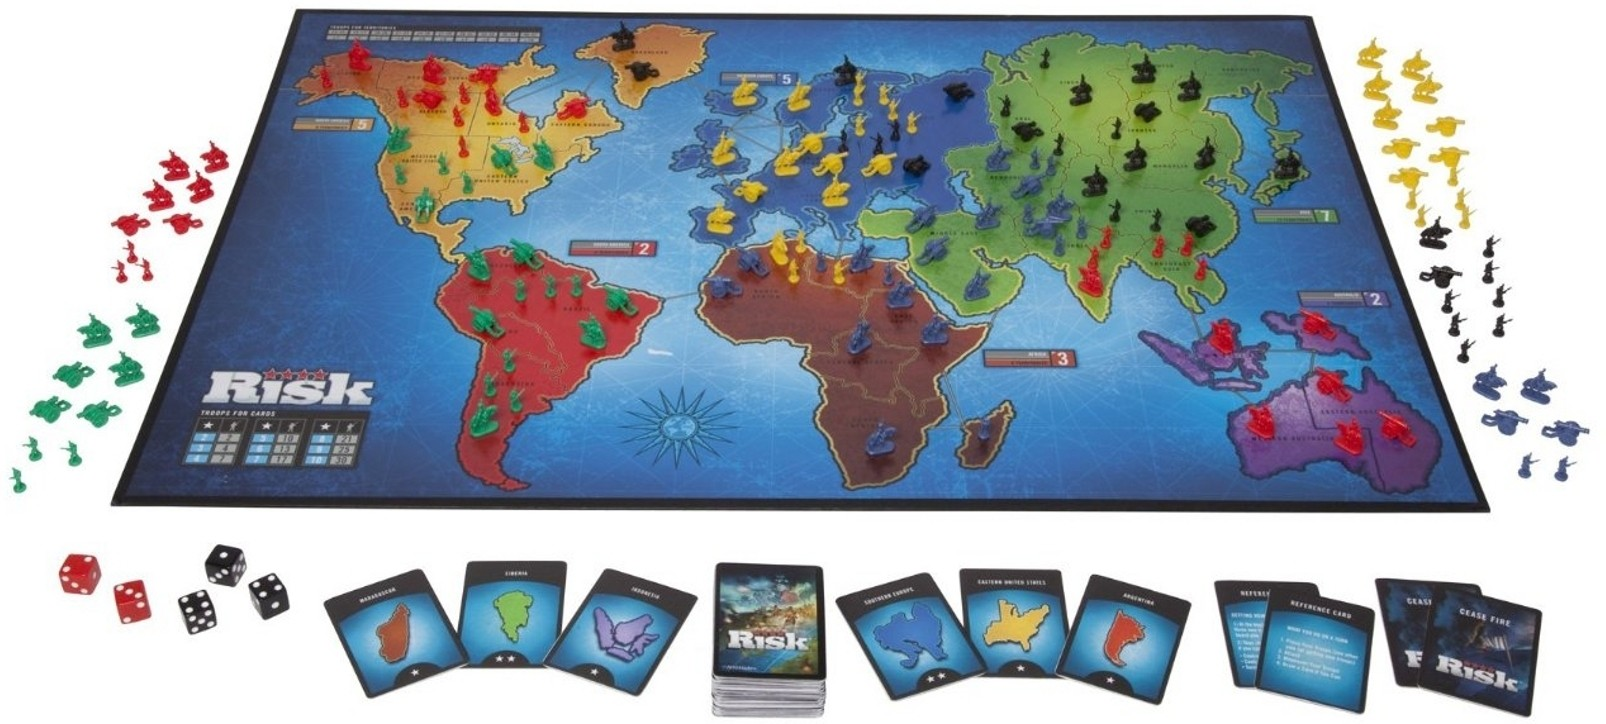
\includegraphics[width=0.21\textwidth]{static/risk}
 \end{center}

 \switchcolumn

\begin{center}
\fontsize{85}{0}\selectfont Cultural evolution
\end{center}

\vspace{1cm}



 
 \begin{center}
 \fontsize{65}{65}\selectfont How \textbf{social behavior} alter
  
  individual \textbf{skill acquisition}? 
 \end{center}

 \vspace{2cm}
 
 \begin{center}
  \includegraphics[width=.225\textwidth]{figures/loyalty}
 \end{center}

 
 \switchcolumn

 
\begin{center}
\fontsize{85}{0}\selectfont Bayesian Inference
\end{center}

 \vspace{1cm}
 
 \begin{center}
 \fontsize{65}{65}\selectfont The way to \textbf{optimally} update
 our \textbf{beliefs}, given a model and data
 \end{center}

 \vspace{2cm}
 
\begin{center}
  \includegraphics[width=0.225\textwidth]{figures/posterior_win}
 \end{center} 
 

\end{paracol}

\vspace{3cm}

\begin{paracol}{3}
%\columnratio{0.25,0.25,0.25,0.25}

 \columnseprule=0pt
 
 \begin{justify}
{\fontsize{55}{0}\selectfont Dataset}
\vspace{1cm}
 \fontsize{43}{50}\selectfont

   We rely a multiplayer \textbf{online game} in which games could be \textbf{played individually or in teams}. Composed by $4.5\times 10^6$ games, $2.0\times 10^5$ users, the \textbf{database is available} at Dryad.  \par

%\hspace{0cm} \textbf{Social learning} is essential for human adaptation. 
%Notwithstanding its importance, the effects of teammate selection was commonly overlooked when studying human learning.
%This gap led us to ask the \textbf{impact} of team play strategies and teammate selection in an online game.
\end{justify}

\vspace{2cm}
\begin{figure}[H]     
     \centering \normalsize 
     \begin{subfigure}[c]{0.07\textwidth}
     \hspace{0.33cm}
        \includegraphics[width=\textwidth]{figures/qr.pdf}
     \end{subfigure}     
        {\fontsize{75}{0}\selectfont \texttt{cor.to/socialLearning} }
\end{figure}


 \switchcolumn
 \begin{justify}
{\fontsize{55}{0}\selectfont Results}
\vspace{1cm}
 \fontsize{43}{50}\selectfont

 We found a \textbf{Faithfulness-boost effect} that provides a skill boost during the first games of experience that individually would only be acquired after thousands of games played.
 
 

 \end{justify}

 
\vspace{3.5cm}

 \begin{justify}
{\fontsize{55}{0}\selectfont Discussion}
\vspace{1cm}
 \fontsize{43}{50}\selectfont

 \textbf{Loyal team-oriented behavior} enable players to early gain individual skills. We suggest that they have \textbf{better access to the cultural information} than alternatives social strategies.
% %people need to be able to fluidly extract and exchange information from the social system. 
 \end{justify}     
 
 \switchcolumn
{\fontsize{55}{0}\selectfont Methods }
\vspace{0.5cm}

\begin{center}
\includegraphics[width=0.2\textwidth]{figures/elo-factor-en.pdf} 
\end{center}


 
 \end{paracol}

 
\end{document}
